
\chapter{ Flugleistungen}

\deftripstyle{Flughandbuch}[.5pt][.5pt]{\pagemark}{}{\headmark}{Flug- und Betriebshandbuch B13}{}{06.2022}
\pagestyle{Flughandbuch}
\renewcommand*\chapterpagestyle{Flughandbuch}


\section{Einführung}
Der vorliegende Abschnitt enthält anerkannte Werte bezüglich Anzeigefehler der
Fahrtmesseranlage, Überziehgeschwindigkeit und Startleistung sowie zusätzliche
andere Werte und Angaben, die keine Anerkennung durch das LBA benötigen.
Die Daten in den Tabellen wurden durch Erprobungsfluge mit einem Motorsegler
in gutem Zustand unter Zugrundelegung eines durchschnittlichen Pilotenkönnens
ermittelt.

\newpage


\subsection{Nachgewiesene Seitenwindkomponenten}
Noch nicht nachgewiesen.
%\begin{tabular}{l l}
%Windenstart: & ?$\frac{km}{h}$\\
%Flugzeugschlepp: & ?$\frac{km}{h}$\\
%Landung: & ?$\frac{km}{h}$\\
%
%\end{tabular}
\section{Geschwindigkeitspolare}
Die Leistungsvermessung der B13 fand im August 1992 in Aalen-Elchingen statt. Die Flugmasse (Rüstmasse + $\unit[180]{kg}$) lag bei $\unit[765]{kg}$, was einer Flächenbelastung von $\frac{G}{S}=\unit[396]{\frac{N}{m^2}}$ entspricht. \\
\newline
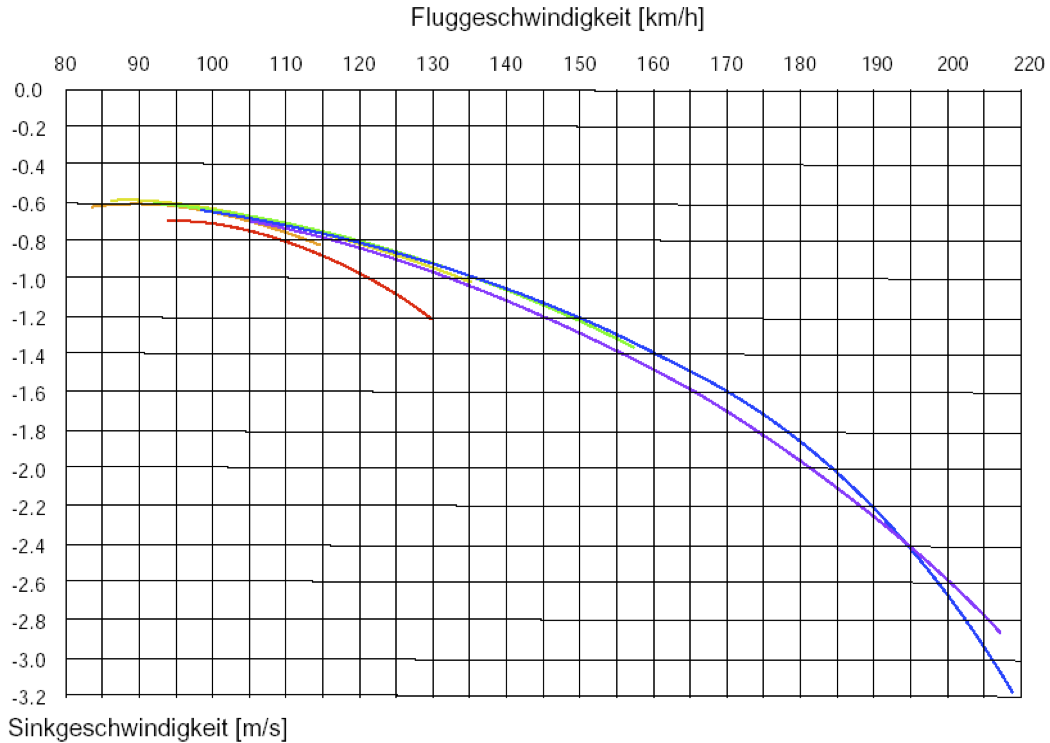
\includegraphics[width=\textwidth]{polare.png}
\newline
\begin{center}
\begin{tabular}{|c|c|c|}
\hline
Wölbklappenstellung & WK-Innen & WK-Außen\\
\hline
\begin{color}{red} L \end{color} & \begin{color}{red} $15,8^{\circ}$ \end{color} & \begin{color}{red} $11,5^{\circ}$ \end{color}\\
\hline
\begin{color}{orange} $+2$ \end{color} & \begin{color}{orange} $10,4^{\circ}$ \end{color} & \begin{color}{orange} $7,5^{\circ}$ \end{color}\\
\hline
\begin{color}{yellow} $+1$ \end{color} & \begin{color}{yellow} $4,5^{\circ}$ \end{color} & \begin{color}{yellow} $3,2^{\circ}$ \end{color}\\
\hline
\begin{color}{cyan} $0$ \end{color} & \begin{color}{cyan} $0^{\circ}$ \end{color} & \begin{color}{cyan} $0^{\circ}$ \end{color}\\
\hline
\begin{color}{blue} $-1$ \end{color} & \begin{color}{blue} $-4,3^{\circ}$ \end{color} & \begin{color}{blue} $-3,2^{\circ}$ \end{color}\\
\hline
\begin{color}{violet} $-2$ \end{color} & \begin{color}{violet} $-9,7^{\circ}$ \end{color} & \begin{color}{violet} $-7,3^{\circ}$ \end{color}\\
\hline

\end{tabular}
\end{center}
\section{Gleitzahlpolare}
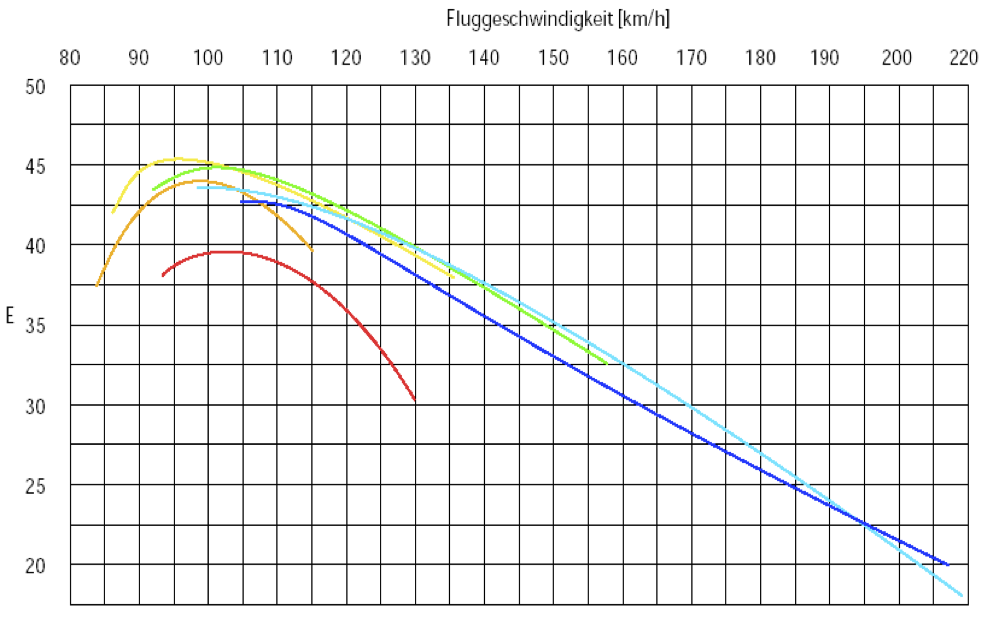
\includegraphics[width=\textwidth]{gzpolare.png}
\newline
\begin{center}
\begin{tabular}{|c|c|c|}
\hline
Wölbklappenstellung & WK-Innen & WK-Außen\\
\hline
\begin{color}{red} L \end{color} & \begin{color}{red} $15,8^{\circ}$ \end{color} & \begin{color}{red} $11,5^{\circ}$ \end{color}\\
\hline
\begin{color}{orange} $+2$ \end{color} & \begin{color}{orange} $10,4^{\circ}$ \end{color} & \begin{color}{orange} $7,5^{\circ}$ \end{color}\\
\hline
\begin{color}{yellow} $+1$ \end{color} & \begin{color}{yellow} $4,5^{\circ}$ \end{color} & \begin{color}{yellow} $3,2^{\circ}$ \end{color}\\
\hline
\begin{color}{cyan} $0$ \end{color} & \begin{color}{cyan} $0^{\circ}$ \end{color} & \begin{color}{cyan} $0^{\circ}$ \end{color}\\
\hline
\begin{color}{blue} $-1$ \end{color} & \begin{color}{blue} $-4,3^{\circ}$ \end{color} & \begin{color}{blue} $-3,2^{\circ}$ \end{color}\\
\hline
\begin{color}{green} $-2$ \end{color} & \begin{color}{green} $-9,7^{\circ}$ \end{color} & \begin{color}{green} $-7,3^{\circ}$ \end{color}\\
\hline

\end{tabular}
\end{center}
\newpage
\section{Leistungsoptimale Wölbklappenbedienung}
Auf Grundlage der Polaren ergeben sich für die verschiedenen Manöver die optimalen Wölbklappenstellungen:\\
\newline
\begin{tabular}{|m{3,5cm}|m{2cm}|m{4cm}|}
\hline
Verwendung & WK-Stellung & Geschwindigkeit [$\unit{\frac{km}{h}}$]\\
\hline
langsames Kreisen in Ruhiger Thermik & $+2$ & $85$ bis $100$\\
\hline
schnelleres Kreisen in der Thermik, bestes Gleiten, geringstes Sinken & $+1$ & $90$ bis $105$\\
\hline
Gleitflug zwischen Aufwinden & $0$ & $100$ bis $135$\\
\hline
Gleitflug mit erhöhter Geschwindigkeit & $-1$ & $130$ bis $195$\\
\hline
schneller Gleitflug & $-2$ & $190$ bis $220$\\
\hline
\end{tabular}\\
\newline
\newline
Bei Erhöhung der Flächenbelastung und der Schräglage im Kreisflug erhöhen sich auch die Geschwindigkeiten.

\section{Nicht LBA-anerkannte weitere Informationen}
\subsection{Flugleistung im motorgetriebenen Flug}
\subsubsection{Steigrate}

\begin{color}{red}
\large{\underline{Warnung}}\\
Diese Werte sind bisher rechnerisch ermittelt:
\end{color}\\

Die maximale Steigrate kann nur für ca. 14 Minuten bei vollgeladenen Akkupacks erreicht werden, da durch die reduzierte Spannung auch die Steigrate sinkt.

Die durchschnittliche Steigrate hängt von vielen Faktoren ab, vor allem aber von der Abflugmasse.

Der maximale Höhengewinn unter Bedingungen der Standardatmosphäre hängt hauptsächlich von der Abflugmasse ab. Für den maximalen Höhengewinn sollte mit einer Leistung von ca. $\unit[20]{kW}$ geflogen werden (nicht maximale Leistung, da das Optimum bei einer geringeren Einstellung liegt).\\ 
Die Steiggeschwindigkeit liegt normalerweise bei $\unit[80-85]{km/h}$ bei positiver Klappenstellung (wie in der Thermik).\\
%Der rechnerische ermittelte Wert ist: $\unit[1100]{m}$ 
Der maximal erflogene Höhengewinn beträgt $\unit[1100]{m}$ in $\unit[14]{Minuten}$ Motorlaufzeit.

\subsubsection{Reiseflug}
Die maximale Reichweite im Reiseflug ist noch nicht ermittelt. 

% noch nicht fertig
\subsubsection{Dienstgipfelhöhe}
Ein Flug in großer Höhe mit einem mit FES ausgestatteten Segelflugzeug ist trotz des niedrigen Drucks kein Problem. Nach den UN-Transportvorschriften müssen die Zellen, die in den FES Akkupacks verwendet werden acht verschiedene Tests bestehen. Es wird eine Höhensimulation durchgeführt, bei der die Zellen bei einem reduzierten Druck von $\unit[11,6]{kPa}$ (ca. $\unit[15.000]{m}$) getestet werden.\\

Die tiefen Außentemperaturen von bis zu $\unit[-20]{^\circ C}$ stellen weder ein Sicherheitsrisiko für
die Akkupacks (die normalerweise wärmer bleiben), noch für andere Komponenten des Antriebssystems dar. Dennoch ist die Leistung der Akkupacks bei tiefen Temperaturen geringer.

\subsubsection{Lärmdaten} 
Die Lärmmesswerte des Motors sind deutlich geringer als die eines vergleichbaren Segelflugzeugs mit Verbrennungsmotor.
Für Hilfstriebwerke gibt es in diesem Rahmen keine Lärmbeschränkungen.\\

Bezüglich des ENL (Engine Noise Level) Signals für Logger:\\
Es wird darauf hingewiesen, dass zur Erkennung des ENL-Signals bei laufendem Motor der Flugdatenlogger im Instrumentenbrett oder vergleichbar nahe an der FES-Einheit angebracht werden muss. Bei einer anderweitigen Positionierung des Loggers im
Cockpit ist ein separater MOP-Sensor wie für andere leise elektrische Motoren anzubringen.
Es sei auf Annex B des IGC Sporting Code verwiesen.

\subsubsection{Elektromagnetische Störungen}
Es konnte kein ungewöhnliches Verhalten der Instrumente durch die Verkabelung die, unter dem Instrumentenbrett verläuft (inklusive Magnetkompass), während des Motorbetriebes oder des Anhaltens festgestellt werden.



